\section*{Over ons}

\begin{minipage}{0.5\linewidth}
	
\includegraphics[width=\linewidth]{FotoFlorent.jpg}
\end{minipage}
\hfill
\vspace{1cm}
\begin{minipage}{\linewidth}
	\textbf{Florent Kegler (514277)} \\
	\textbf{Rol:} Bedrijfscontact \\
	Ik ben 21 jaar en woon mijn hele leven in Rijssen. Ik heb de opleiding Mechatronica gevolgd aan Saxion University in Enschede. Binnen dit project neem ik de rol van bedrijfscontact op mij. Dat betekent dat ik verantwoordelijk ben voor het onderhouden van het contact met de bedrijven die we tijdens onze studiereis in het buitenland zullen bezoeken.
\end{minipage}

\vspace{1cm}

\begin{minipage}{0.5\linewidth}
	
\includegraphics[width=\linewidth]{FotoTristan.jpg}
\end{minipage}
\hfill
\vspace{1cm}
\begin{minipage}{\linewidth}
	\textbf{Tristan van Duuren (480101)} \\
	\textbf{Rol: } Coördinator activiteiten \& logistiek \\
	Ik ben Tristan van Duuren, 24 jaar oud en ik kom uit Denekamp. Voorafgaand aan BK5 heb ik Bouwkunde gestudeerd aan het Saxion en heb ik een half jaar gewerkt als BIM-modelleur voor een architectenbureau. In de commissie ben ik verantwoordelijk voor het coördineren van de activiteiten en de logistiek. Ik zorg er na goedkeuring van de commissieleden voor dat we op bestemming komen, een geschikte accommodatie hebben en dat er, waar nodig, activiteiten georganiseerd zullen worden. 
\end{minipage}

\begin{minipage}{0.5\linewidth}
	
\includegraphics[width=\linewidth]{FotoStijn.jpg}
\end{minipage}
\hfill
\vspace{1cm}
\begin{minipage}{\linewidth}
	\textbf{Stijn van Straaten (493809)} \\
	\textbf{Rol: } Penningmeester \\
	Ik ben 23 jaar en ik kom uit Goor. Ik heb de hbo opleiding werktuigbouwkunde aan hogeschool Saxion in Enschede afgerond. Voor de buitenlandreis vervul ik de rol van penningmeester. Hierdoor ben ik verantwoordelijk voor het beheren van de financiën en het bewaken van het budget. Ik houd het budget bij, zorg dat alles netjes wordt vastgelegd en verzorg de financiële administratie.
\end{minipage}

\vspace{1cm}

\begin{minipage}{0.5\linewidth}
	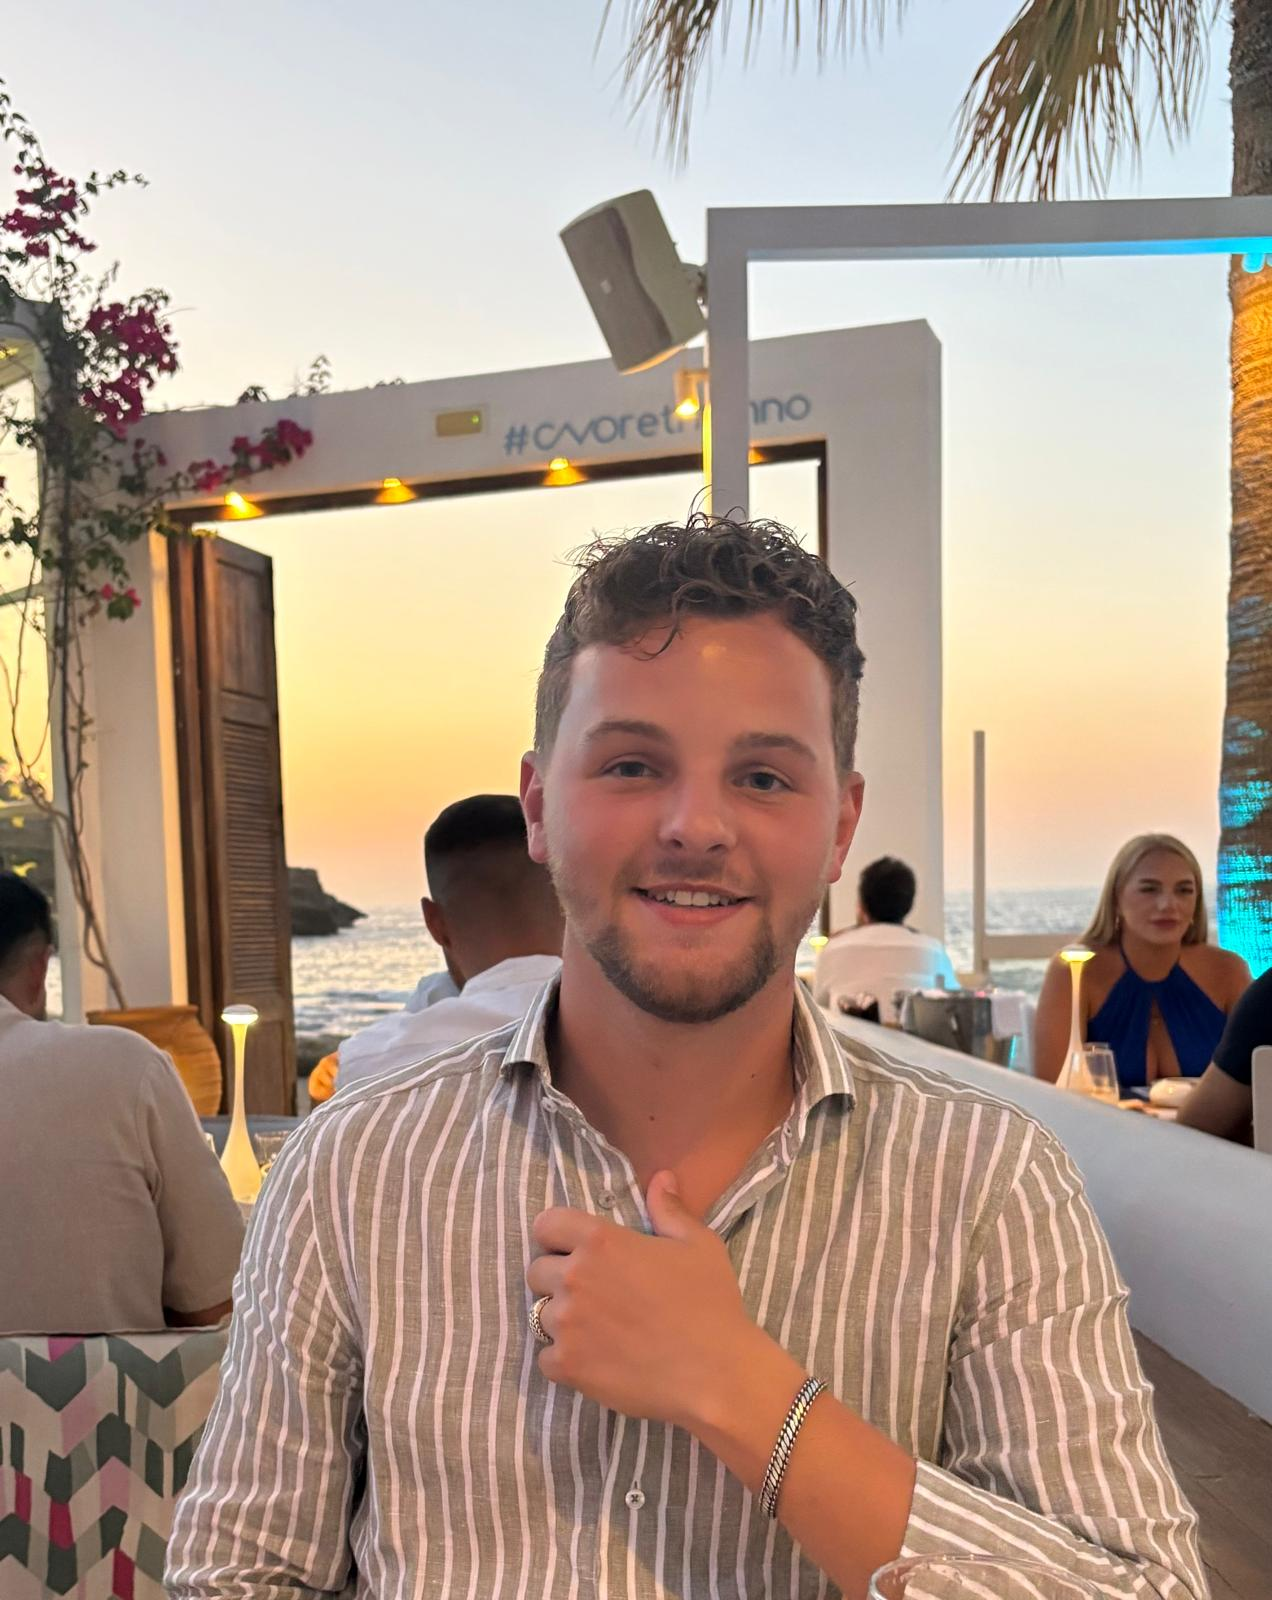
\includegraphics[width=\linewidth]{FotoMarijn.jpg}
\end{minipage}
\hfill
\vspace{1cm}
\begin{minipage}{\linewidth}
	\textbf{Marijn van der Gracht (499194)} \\
	\textbf{Rol:} Voorzitter \\
	Ik ben Marijn van der Gracht, 23 jaar oud en kom uit Hengelo. Ik heb voorafgaand aan de studie BK5, mechatronica gestudeerd aan de Hogeschool Saxion in Enschede. Voor het komende schooljaar vervul ik de rol van Voorzitter in de buitenlandreis commissie. Van mij wordt verwacht dat ik sturing geef aan mijn naaste commissie genoten en communiceer met het bestuur. Ook houd ik rekening met de wensen van de aangesloten studenten bij onze studiereis, zodat iedereen een prettige studiereis heeft. 
\end{minipage}